\documentclass[letterpaper, 10 pt, journal, twoside]{IEEEtran}
%\documentclass[journal]{IEEEtran}
\usepackage[maxnames=6,firstinits=true,doi=false,url=true,isbn=false]{biblatex}
\addbibresource{IROS.bib}
\usepackage{array}
\usepackage{graphicx}
\usepackage{amsmath}
\usepackage{amssymb}
\usepackage{color}
\usepackage{threeparttable}
\usepackage{balance} %balance columns
\usepackage{todonotes}
\hyphenation{op-tical net-works semi-conduc-tor}
%\usepackage[colorlinks]{hyperref}
\usepackage{breakurl}

%\pagenumbering{gobble} %suppresses page numbers

\begin{document}
\title{A Multi-Agent Systems Approach to Test Generation for Simulation-based Autonomous Vehicle Verification}
\author{Greg~Chance$^{1}$, 
Abanoub~Ghobrial$^{1}$, 
Severin Lemaignan$^{2}$,
Tony Pipe$^{2}$,
Kerstin Eder$^{1}$%~\IEEEmembership{Senior Member,~IEEE}, 


%\thanks{Manuscript received: Feb 23, 2018; Revised: May 21, 2018; Accepted: Jun 21, 2018.}
\thanks{$^{1}$Abanoub Ghobrial, Greg Chance and Kerstin Eder are with the University of Bristol, Bristol, UK {\tt\footnotesize \{greg.chance, abanoub.ghobrial, kerstin.eder\}@bristol.ac.uk}}%
\thanks{$^{2}$Severin Lemaignan and Tony Pipe are with the Bristol Robotics Laboratory, University of the West of England, Bristol, UK {\tt\footnotesize \{severin.lemaignan, tony.pipe\}@brl.ac.uk}}%
}
% The paper headers
%\markboth{Submission to IEEE AI Testing 2019}%
%{Shell \MakeLowercase{\textit{et al.}}: Bare Demo of IEEEtran.cls for IEEE Journals}
%\markboth{IEEE Robotics and Automation Letters. Preprint Version. Accepted June, 2018}
%{Chance \MakeLowercase{\textit{et al.}}: ``Elbows Out" - Predictive Tracking of Partially Occluded Pose} 
\maketitle

\begin{abstract}
Simulation-based verification is beneficial for assessing otherwise dangerous or costly on-road testing of autonomous vehicles (AV). This paper addresses the challenge of efficiently generating effective tests for simulation-based AV verification using software testing agents. The multi-agent system (MAS) programming paradigm offers rational agency, causality and strategic planning between multiple agents. We exploit these aspects for test generation, focusing in particular on the generation of tests that trigger the precondition of an assertion. On the example of a key assertion we show that, by encoding a variety of different behaviours respondent to the agent's perceptions of the test environment, the agency-directed approach generates twice as many effective tests than pseudo-random test generation, while being both efficient and robust. Moreover, agents can be encoded to behave naturally without compromising the effectiveness of test generation. Our results suggest that generating tests using agency-directed testing significantly improves upon random and simultaneously provides more realistic driving scenarios.
%
%Our results suggest that generating tests using testing agents allows engineers to reach edge cases and rare events more easily. %
% GC:

% Simulation based verification for autonomous vehicles (AV) is beneficial for assessing otherwise dangerous or costly on-road testing. The multi-agent system (MAS) programming paradigm was used in the context of AV verification to explore the potential for test generation. Generating tests using autonomous agents has many benefits including scalability and engineering efficiency. We explore different agent behaviours towards the goal of assertion coverage through a simple example. By provoking behaviours based on the agents perceptions of the scenario we show that the agent-based test generation out-performs random agent actions by over 50\% in terms of test generation accuracy. MAS test generation shows promising results for simulation based verification allowing engineers to exploit edge cases and rare events more easily. 

\end{abstract}
\begin{IEEEkeywords}
Test Generation, Simulation, Autonomous Driving, Verification, Multi-Agent System, Test Agent
\end{IEEEkeywords}
\IEEEpeerreviewmaketitle

%------------------- Intro -----------------------------
\section{Introduction}\label{s:introduction}
%\IEEEPARstart{A}{n} agent is a computational mechanism that exhibits a high degree of autonomy, performing actions in its environment based on information received \cite{Panait2005}. A multi-agent system contains one or more agents whom interact but may not share information about the environment that is known by a single agent. This individual level information bias may lead to emergent properties in the multi-agent group behaviour as a result of the interaction between agents.

%----------------------------------------------------------
% What is verification
\IEEEPARstart{V}{erification} is the process used to gain confidence in the correctness of a system with respect to its requirements~\cite{bergeron2012writing}. Testing is a technique that can be used to achieve this by showing that the intended and actual behaviours of a system do not differ and detecting failures against the requirements in the process~\cite{utting2012taxonomy}.



%----------------------------------------------------------
% What is the role of testing
% above
% Actual quote is: "Verification is a process used to demonstrate that the intent of a design is preserved in its implementation", [Bergeron].

%----------------------------------------------------------
% The principle of verification based testing
Using simulation to test autonomous driving functions in safety critical scenarios benefits from full control over the environment, where road layouts, weather conditions, a variety of road users and other %traffic participants
driving scenario parameters 
can be directed to achieve specific test targets. %
%
% These tests may look to convince auditors of the functional safety of the vehicle or whether it complies with commonly agreed upon road conduct, such as the Vienna convention~\cite{ViennaConv}, interpreted locally by each country, e.g.\ the UK Highway Code~\cite{codes2011highway}. In addition, there are also road traffic laws and penalties, e.g.~\cite{RoadTraffic1988}, and unwritten rules or social conventions~\cite{}. 
%
These tests may aim to provide evidence to regulators of the functional safety of the vehicle or its compliance with commonly agreed upon road conduct, such as the Vienna convention~\cite{ViennaConv}, typically implemented at national level as a set of rules~\cite{codes2015highway}, road traffic laws and penalties~\cite{RoadTraffic1988}.
%
%These may be culturally or geographically different, e.g.\ flashing headlights to override junction priorities to give way to another driver.


%----------------------------------------------------------
% The Test Generation challenge and its automation
Verification of complex systems is challenging. In semiconductor design, for
example, it has long been recognised that verification can take up to 70\% of
the design effort~\cite{arden2002international}, with the largest part still
being achieved with simulation-based techniques. 
%
The testbench is the code used to drive a stimulus sequence into the Design
under Verification (DUV) while observing input protocols. It also records
coverage and checks the DUV's response. The testbench provides a completely
closed environment from the DUV's perspective. Simulators are used to execute
testbenches. Automation plays a critical role in achieving verification targets
efficiently and effectively.

Coverage-driven verification is a systematic, goal-directed simulation-based
verification method~\cite{HVC2015} that offers a high degree of automation and
is capable of exploring systems of realistic detail under a broad range of
environment conditions.
%
Because exhaustive simulation is intractabe due to the vast parameter space,
the remaining challenge is in strategically selecting the (ideally smallest set
of) test cases that result in the highest level of confidence in the design's
correctness.
%
Automating test generation has been the focus of research for decades, giving
rise to a variety of coverage-directed stimulus generation techniques that
exploit formal methods, genetic programming and machine learning~\cite{Ioannides:2012}. 

Compared to semiconductor design verification, AV verification faces even bigger challenges, including automatic test generation. 
%
It is well known that few of the valid tests are actually interesting from a verification point of view. 
Estimates vary, but demonstrating AV safety with a confidence of 95\% that the failure rate is at most 1.09 fatalities per 100 million miles driven would take 275 million miles, equivalent to 12.5 years for a fleet of 100 AVs~\cite{kalra2016driving}. %
%
This figure is based on the number of roads fatalities in the US, and would
need to be adjusted taking into consideration local statistics on road safety,
e.g.\ the number of road fatalities per billion vehicle-km in the UK has been
half that of the US in 2018~\cite{ITFroadSafety2018}.
%
Ways must be found to test the scenarios of interest without needing millions of miles of driving or billions of miles of simulated driving~\cite{korosec2019waymo}.
%
In particular, simulation-based testing offers the opportunity to increase the number of otherwise rare events~\cite{Koopman2018} in order to determine whether the AV handles such rare events appropriately. 
%
% For the public to gain trust in autonomous vehicles (AV), the manufacturers must demonstrate that their AVs comply with, amongst many things, road safety requirements. 
% While on-road testing will contribute significantly towards AV verification, testing in simulation has complimentary benefits as it offers a safe and effective environment. 
%
% Testing in simulation enables many processes to be automated which may be convenient for ensuring compliance during version change, e.g. software updates or patches to the vehicle.
% But automation can also apply to not just the process but the method of test generation which is the focus of this paper.


\begin{figure}[!t]
	\centering
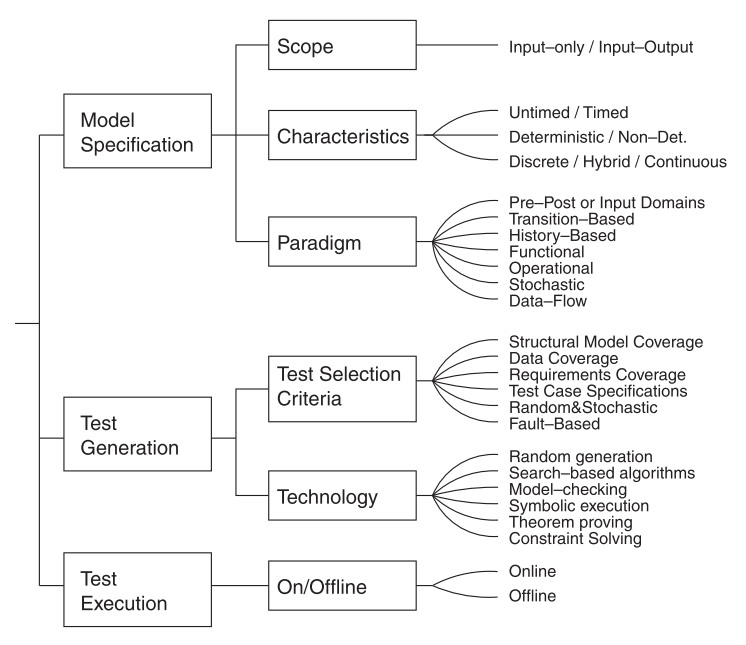
\includegraphics[width=0.48\textwidth]{taxonomy.png}
	\caption{Taxonomy of model-based test generation, from~\cite{utting2012taxonomy}.}
	\label{f:taxonomy}
\end{figure}


%----------------------------------------------------------
% The AV as a DUT/SUV/DUV
Considering the AV as a DUV, the challenge is to generate tests that interact with the AV over a period of time, thereby creating an environment in which the AV needs to respond to the received stimulus while making progress towards its destination. 
%
As such, the AV can be classed as a \textit{responder\/} DUV, i.e.\ a DUV that reacts to lower-level stimulus observed on its interfaces with the surrounding environment in order to maintain legally correct driving behaviour and follow the social norms associated with road traffic.
%
% RESPONDER (https://verificationacademy.com/cookbook/doc/glossary/responder): A verification component which, similar to a driver, interacts with a lower level of abstraction such as the individual signals on a protocol interface, in order to participate in a protocol. Unlike a driver, responders do not initiate stimulus traffic from a sequence, they respond (slave-like) to traffic observed on the interface in order to maintain legal protocol. Their execution may be controlled by configuration (specifying how they are to respond in general) including some constrained randomization possible within the allowed configuration space, or by sequences of configuration changes (altering the way they respond in a controlled way), or by maintaining some state, e.g. a memory model or register model, which reflects persistent data values deposited by earlier traffic and subsequently retrieved accurately by the responder.
%
%----------------------------------------------------------
% The promise of AGENCY to address verifying responders
This paper investigates the benefits of introducing \textit{agency} into the verification environment in order to address the challenges of verifying the responder DUV. 
%
Each software agent is tasked with specific goals that aim to achieve verification objectives, e.g.\ reaching coverage targets.
%
A set of software agents can then be directed to interact, coordinating their behaviour in response to the AV's observed actions in order to increase the likelihood of rare events occurring during simulation to reach coverage targets faster.
%
%----------------------------------------------------------
% Research Questions
% -new test generation technique
Our key research question is: what are the benefits of using agent-based test generation for the verification of AVs in simulation?
%
In particular, we are interested in how agency-directed test generation compares to pseudo-random test generation techniques wrt.\ the following criteria for a 'good' test case, which are inspired by~\cite{fewster1999software}:
%
%----------------------------------------------------------
% What makes a good test case?
% The challenge here is to find the correct stimulus for the AV which is described by the test case. 
%
\textit{effectiveness} in detecting failures, 
\textit{efficiency} in minimising the number if tests required to achieve verification goals, 
\textit{economy} in terms of resource usage % during verification as well as during the analysis of the verification results, 
and also 
\textit{robustness} towards changes. 
%
Our results suggest that generating tests using directed agents significantly improves upon random and simultaneously provides driving scenarios that are more realistic than those obtained by random test generation.

We regard agent-based test generation as a contribution to the well-established model-based test generation paradigm. A taxonomy of model-based test generation from~\cite{utting2012taxonomy} is given in Figure~\ref{f:taxonomy}.
%
The agent-based technique creates two new entries in that taxonomy, a new Paradigm under Model Specification, \textit{Agent-based}, and a new Technology under Test Generation, \textit{Agency}, which includes reactive reasoning, causality and strategic planning between multiple agents.
%
In this paper we use an agent-based model to specify the test environment of the AV. Agency is given to the key dynamic entities in the test environment that interact with the AV, in our case pedestrians. Agency, implemented through a belief-desire-intention agent interpreter such as Jason~\cite{bordini2005jason} is then employed to generate tests based on the multi-agent system that represents the test environment. Note that other test generation techniques, such as random generation, which we use as baseline for evaluation, or model checking~\cite{Bordini2006}, can also be applied to an agent-based model.	

This paper is structured as follows. In the next section we introduce the terminology we will adopt throughout the paper and present the testbench architecture used in our experiment. In Section~\ref{s:background} we review related work on test generation for simulation-based AV verification and introduce the basics of multi-agent systems. Section~\ref{s:case-study} presents our case study, which is centred around test generation for a collision avoidance scenario. Results are presented in Section~\ref{s:results} and evaluated in Section~\ref{s:evaluation}. We conclude in Section~\ref{s:conclusion} and give an outlook on future work. 

\section{Terminology and Testbench Architecture}\label{s:testbench}
%----------------------------------------------------------

%----------------------------------------------------------
% Scene, Scenario definitions
We will adopt the terminology defined in~\cite{Ulbrich2015}, where \textit{scene} refers to all static objects including the road network, street furniture, environment conditions and a snapshot of any dynamic elements. Dynamic elements are the elements in a scene whose actions or behaviour may change over time, these are considered actors and may include other road vehicles, cyclists, pedestrians and traffic signals. 
%
The \textit{scenario} is then defined as a temporal development between several scenes which may be specified by specific goals and values.
%
A \textit{situation} is defined as the subjective conditions and determinants for behaviour at a particular point in time. 

% Test Bench Architecture
The proposed testbench, see Fig.~\ref{f:testbench}, is driven by a specification for the experiment which defines the scene and scenario including all dynamic actors. 
%
The experiment or test case specification specifies the test inputs, i.e.\ the execution conditions for an item to be tested~\cite{StandardsBoard1990}.
%
The vehicle behaviour interface (VBI) connects the AV controller (vehicle control) to the simulator. It provides the simulator with the driving decisions of the AV and forwards updates on the scene to the AV controller. 
%
A geospacial database logs the AV and all other actors to enable post-simulation assertion checking. 


\begin{figure}[!t]
	\centering
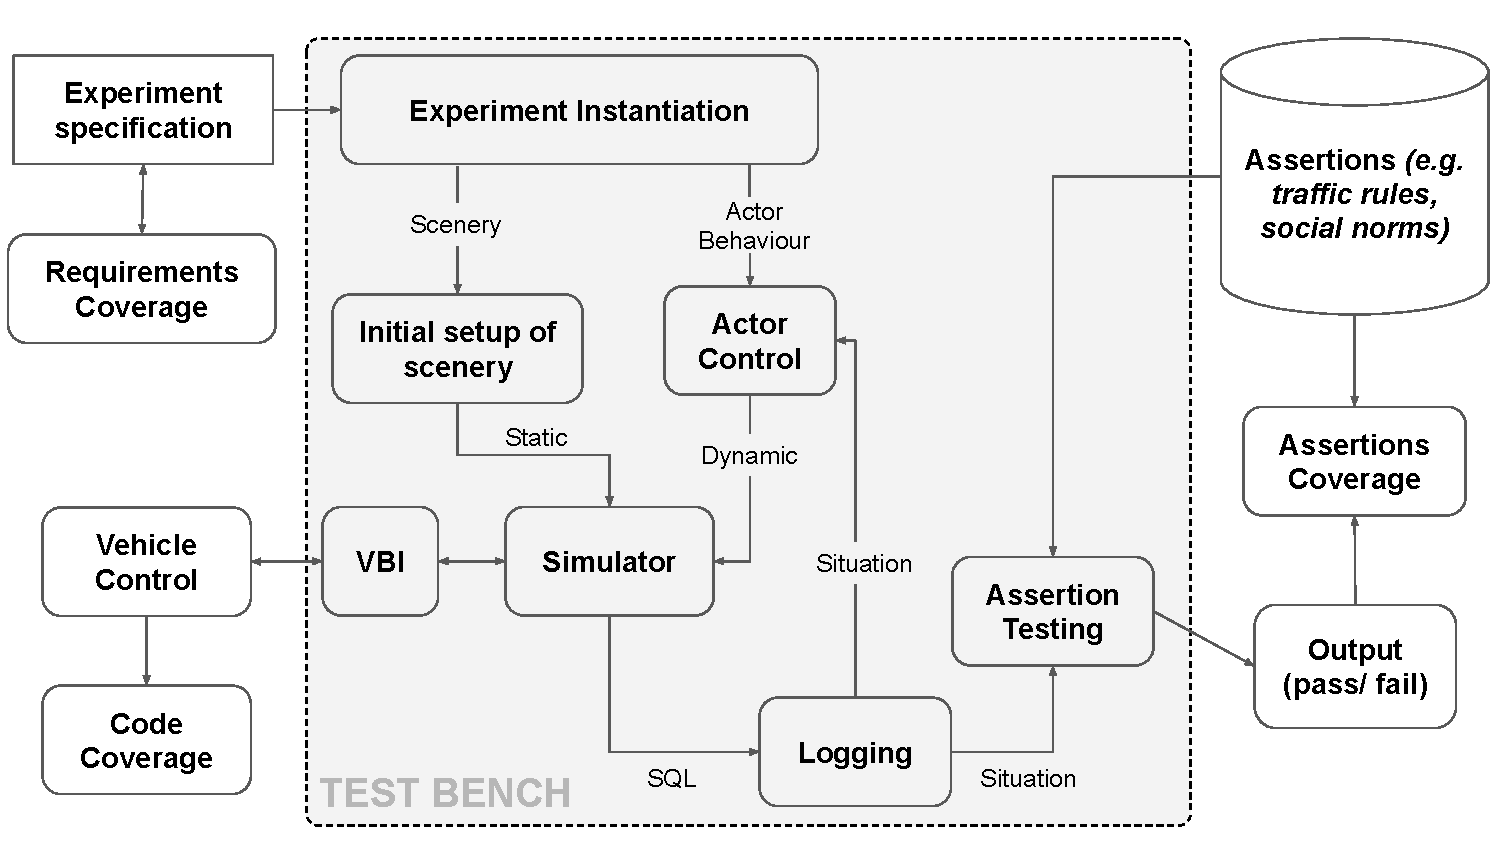
\includegraphics[width=0.48\textwidth]{TestBenchMonotone.pdf}
	\caption{Testbency Architecture.}
	\label{f:testbench}
\end{figure}

%
Given the experiment specification, tests may be generated in a variety of ways that differ mainly in their effectiveness and efficiency. 
%
Manually generated tests are typically effective in achieving verification objectives, but are considered expensive due to the high engineering cost involved. 
%
Random methods are usually employed at the early stages of testing to build up coverage quickly. They suffer, however, from a high number of invalid tests being generated and, even when constrained to produce only valid tests, the tests generated are often not interesting wrt.\ the verification objectives, in our case this refers to exercising the collision avoidance decision making logic of the AV. 
%
Model-based test generation offers an alternative that produces valid and interesting tests at the cost of developing a model that faithfully encodes the behaviour of the test environment. This model can then be explored in a variety of ways, see Figure~\ref{f:taxonomy}.
%
%----------------------------------------------------------
% Summary
Our paper explores how the agency that is naturally present in the multi-agent system that represents the dynamic actors in a scene can be used for model-based generation of test scenarios in the context of simulation-based AV verification. 

% \todo[inline]{Natural = waiting for interesting event, Edge case = find only interesting events.}
One could argue that the simulation environment presented to the AV should be as close to the real world it seeks to emulate as the most realistic proving ground. Such efforts seek to reduce the \textit{reality gap}, %~\cite{Jakobi1995} 
providing the most likely scenarios and actor behaviour. This can be achieved by monitoring real traffic scenarios, e.g.\ tracking individual vehicles, cyclists and pedestrians, and building behavioural models for each of the tracked entities~\cite{behbahani2019learning}.
%
On the other hand, the creation of edge cases is critical to reach verification objectives in a timely manner. Edge cases are events that occur rarely under normal circumstances, yet realistic \textit{and\/} critical for gaining confidence in the correct behaviour of the AV.
%
This is exactly what the agent-based test generation approach introduced in this paper is aimed at.  


\section{Background}\label{s:background}

%------------------- Related -----------------------------
\subsection{Related Work}\label{s:background}
% Describe conventional methods for test generation for verification, e.g. formal methods, random methods, hand-written tests.
% Discuss the ways that you can generate tests 1)use random 2) use engineers to write tests 3)AI/ML methods ...

An overview of the challenges currently faced in software testing of AVs is given by Koopman, highlighting the importance of fault injection into the testing domain~\cite{Koopman2016} and how to decide what aspects of the system need to be tested in the areas of operational design domains, event detection and vehicle manoeuvres~\cite{Koopman2019}. 
%
Describing a driving scene in natural language has been shown to be an effective framework for scenario generation. This can also be automated based on formalised rules and knowledge~\cite{Bagschik2018} or even evolved from ISO safety standards~\cite{Menzel2018}. 
%
Hallenbach et al.\ take the approach to test generation of developing composite metrics for traffic quality and using them to determine if a scenario is `critical' or not and therefore worth exploring further~\cite{Hallerbach2018}. 
%
Generating targeted test cases can be a more efficient way to achieve verification objectives. 
%
For example, Mullins et al.~\cite{Mullins2018} describe a test generation method that is focused on exploring the transitions between decision making performance modes of the AV, with the aim to find tests that exercise the complete decision making logic. 
%
Saigol et al.~\cite{Saigol2018} discuss the need for \textit{smart actor control} which they expect may lead to interesting scenarios when these interact with the AV a testbench framework for automated testing. 
%
Rocklage et al.~\cite{Rocklage2017} approach the problem of test generation from the viewpoint of the other traffic participants, using a trajectory planner to ensure coverage over a fixed list of scene parameters. 
%
Tuncali et al.,~\cite{Tuncali2019} use rapidly exploring random trees to explore boundary scenarios for different adversarial road users.
%
Exploiting agency for test generation, however, has not yet been investigated. 

% There are many factors that may influence the choice of test generation for your application, here we choose to focus on accuracy and cost, see~Fig\ref{cost_accuracy}. Accuracy in this context is defined as the ratio of tests that exercise the targeted assertion compared to the total number of tests generated. In another way this is the efficiency of the test generation method in 'finding' coverage.

% Cost in this context is defined as either computational costs or time put in to write the test by a verification engineer. As shown in Fig\ref{cost_accuracy}, some methods may be relatively low cost with low accuracy such as a random method. Random based methods are very popular for AV verification (refs) with the idea being that enough low probability events over millions of miles of testing will give auditors the confidence that enough corner cases have been experienced.

% The other end of the spectrum takes us to hand written tests by verification engineers or those with vested interests in specific scenarios, e.g. a local authority assessing safety of a new road layout. The test case written by the engineer will almost certainly achieve the desired coverage point but at a much higher cost than a random method.


%----------------------------------------------------------
% MAS background and use of MAS for TG (morse, norway - in email from KE)
\subsection{Multi-Agent Systems}

Georgeff and Lansky were key in the development of the belief-desire intention (BDI) agent programming approach~\cite{georgeff1987reactive} and also in the early work of multi-agent systems~\cite{georgeff1988communication}.
%
In a multi-agent system, multiple intelligent agents interact in order to collectively solve problems that are too difficult or impossible for individual agents to achieve. 
%
A multi-agent system includes a set of software agents and their environment. Agents can be equipped with varying degrees of agency, starting from  passive agents, such as obstacles, including active agents that have goals of low complexity, such as pedestrians that act as part of a group, to rational agents that are capable of reasoning based on a cognitive model of the situation, their perception of the surrounding environment, and a set of rules they can use for strategic planning and communication with other agents in the system.
%
The individual agents are considered \textit{autonomous} and in control of their behaviour within the multi-agent system as they pursue their goals. 
% 
This results in self-organisation and self-direction towards achieving a common goal. 

%Waters et al. describe improvements to BDI agents through modifying the intention selection method using priority-based schedulers. They propose \textit{enablement checking} where an agent should not attempt to pursue an intention if there is no way to accomplish it and claim substantial benefits can be gained when 'running vulnerable programs in dynamic environments'~\cite{Waters2015}. This is an interesting approach and highly relevant to the AV verification domain potentially preventing unwanted emergent agent behaviour such as 'zombie attack'.
%
%Schut et al. argue that the intentions of a rational agent are not static and should reconsider their intentions if they cannot be acted upon~\cite{Schut2004}. Considering the degree of inaccessibility of the goal and cleverly considering intention reconsideration as an action the authors use POMDP to find the optimal intention reconsideration policy. Faccin et al. propose higher level intention selection using a meta-model to learn and predict plan outcomes~\cite{faccin2015bdi} demonstrating positive experimental results.
%
%----------------------------------------------------------
% Automated TG
%Automatically generating stimulus that will increase functional coverage is a key challenge in simulation based verification and is a key virtue of constrained pseudo-random techniques. But such techniques are also far from completely automated, as the verification engineer must supply the suitbale constriants which become ever more complex in real driving scenarios. Feedback based coverage-driven generation (CDG) employs machine learning techniques to automatically generate tests based on rewards from a neural network or Markov Decision Process (MDP). Inductive Logic Programming based Coverage Driven Generation (ILP-CDG) has been shown to improve coverage closure by training on data generated during psuedo-random test generation and learning rules to constrain subsequent simulations~\cite{Eder2007}.

%----------------------------------------------------------
% MAS Automated TG
Combining the BDI framework with an automated test generation approach leads to the concept of a software agent capable of generating tests.
Such intelligent, agent-based test generation has first been applied in the human-robot interaction domain~\cite{Araiza-Illan2016}, where a coverage-driven test generation approach was supplemented with reinforcement learning to improve the efficiency and effectiveness of testing the critical part of a robot-to-human handover task within a collaborative manufacturing scenario. 
%
Test agents have also been proposed by Enoiu et al.~\cite{Enoiu2019} for regression testing, although they are used more for test selection from a library of tests, rather than for test generation. These agents use inter-agent messaging to decide what tests to execute and with what prioritisation.
%
%----------------------------------------------------------
% MAS Automated TG

% Hawkins et al.~\cite{hawkins2019situation} use the Multi-Agent Simulator Of Neighbourhoods (MASON) platform to filter tests wrt.\ situation coverage from a small model for an autonomous robot to efficiently ensure parameter combinations are not repeated.


%----------------------------------------------------------
% lead from MAS background into literature

%------------------- Problem -----------------------------
% \section{Problem and Hypothesis}

% We want to verify the AV's suitability for deployment on the road by testing the autonomous driving functions against a set of assertions that an auditor or regulator may take as part of a body of evidence to assess the vehicle's safety case.

% To gain trust the AV must demonstrate its ability to make the right decision and, as discussed in~\cite{koopman}, for the right reason, although we will not go to that level of assessment in this paper. So how do we gain trust in this context? On-road testing is an obvious start and an essential part of testing albeit the most costly and time consuming. Testing in simulation is an appealing route many are now considering~\cite{refs} due to the level of control and alleviates many safety related restrictions to the type of tests that can be undertaken. There are the brute-force approaches to simulation~\cite{ref} where verification is sought simply through a high number of driven miles which has been estimated should be in the millions~\cite{ref} if not hundreds of millions~\cite{ref} and requiring substantial computing resources to complete within a 1-2 month time-frame~\cite{ref}.

% Do we discuss model-based test gen? Or formal methods? \todo[inline]{both, so we can compare}

% Generating targeted test cases can be a more efficient way to get complete coverage for the system. By finding tests that exercise the complete decision making domain we can do away with 'unnecessary miles' of testing.

% The next level would be agents that can act on multiple assertions and their intention selection is a feedback controlled from the coverage checker.
% This is done to assess that the test generation conception can generate valid tests and how this compares to random based techniques.




% =======================================================
%------------------- Method -----------------------------
\section{Case Study} \label{s:case-study}
 
This section describes a case study to explore the proposed agent-based test generation method.%
\footnote{The code used is available at \url{github.com/TSL-UOB/CAV-MAS}.} %
%
Our aim is to generate tests that exercise an assertion that requires the AV to avoid collisions with other road users, provided that such road user, a pedestrian in this case, intrudes in the path of the AV in such a way that a collision can be avoided by the AV either by braking or manoeuvring. In Fig.~\ref{gridRoad} this is illustrated by the \textit{precondition zone}, i.e.\ the area of interest in which the assertion is activated.

In the following, we shall term tests that activate the assertion \textit{successful tests}; these count towards assertion coverage. 
%
% The precondition is activated when an entity (pedestrian) intrudes in the path of the AV which can be avoided either by braking or manoeuvring, see the `Precondition Zone' in Fig.~\ref{gridRoad}. 
Intrusions that fall within the \textit{stopping distance} of the AV~\cite{codes2015highway}, i.e.\ the 12m long zone 
directly ahead of the AV when driving at 30km/h, equivalent to {\raise.17ex\hbox{$\scriptstyle\sim$}}20mph (miles per hour) as marked in Fig.~\ref{gridRoad}, are not considered interesting as they result in unavoidable collisions; tests of this type are of limited use~\cite{Tuncali2018}. 
%
%\todo{Check this!}
Thus, in this case study, unavoidable collisions are those with a time to collision (TTC) of less than 1.33s. The extent of the \textit{precondition zone} is limited to a single simulation tick (1.0s) which puts the upper limit at 2.33s ahead of the \textit{stopping distance}.% based on 12m
%
% KIE: an avoidable collision is defined as TTC<1s - REALLY? THIS WOULD BE FOR 9m, rather than 12m stopping distance :(

A single assertion is chosen so that we can study the fundamental properties of agent-based test generation in a simple setting in comparison to using random test generation techniques.
%
Moreover, in this investigation we do not consider the test result (pass or fail), i.e.\ the behaviour of the AV in response to the assertion being activated. 


%------------------- Test Environment -----------------------------
\subsection{Test Environment}
The test environment, depicted in Fig.~\ref{gridRoad}, is a straight two-lane 99m road with two 6m wide lanes. Pavements are on both sides of the road which are three meters in width giving a total area of 18m$\times$99m. 
%
The AV velocity is 9.0m/s (equivalent to {\raise.17ex\hbox{$\scriptstyle\sim$}}20mph) and the pedestrian velocity is 1.4 m/s (equivalent to {\raise.17ex\hbox{$\scriptstyle\sim$}}3mph). The map is discretised with 1.5m resolution for simple division into the AV and pedestrians' velocities. Thus, in the discretised world the AV velocity is 6 cells/s and the pedestrians' velocity is roughly 1 cell/s. The total number of map cells is 12$\times$66 = 792 cells. 

The AV travels along the left-hand lane of the road starting at cell $y=0$ and travelling to the end, cell $y=66$. If the assertion is triggered
% KIE: Does this mean activated (i.e.\ precondition satisfied) or it fires, i.e. the postcondition is not satisfied?
 or the AV reaches the end of the road, then the test is restarted. The AV occupies an area 4.5m$\times$3m equivalent to 3$\times$2 cells. There are no other vehicles and the right-hand side of the road is unoccupied.

To activate the assertion, the precondition must be satisfied, i.e.\ an agent has entered the \textit{precondition zone} of the AV, which extends 6 cells forwards of the \textit{stopping distance} of the vehicle as shown in~Fig.~\ref{gridRoad}. 
%
Under the given conditions, it is impossible for an agent to move into the AV's path from some pavement areas within the test environment. These are marked in dark grey in Fig.~\ref{gridRoad} and labelled invalid spawn locations. 

The environment is initialised with the agents spawned randomly on any valid spawn location within the pavement area. When the environment is reset, new random locations are chosen for the agents. Random locations are controlled by using a fixed seed that is based on the experiment number; thus, initial spawn locations become repeatable (through using the same seed), which ensures a fair comparison between different experiments.

 %On the left hand-side of the left pavement a pedestrian needs to move three cells to the right to reach the left part of the centre of the left lane. This is equivalent to three seconds. In this time the AV crosses 18 units. Therefore, the first 18 cells of the left-hand side of the left pavement are dead-zone where pedestrians cannot intersect the car if spawn inside this zone. Similarly, the first 12 cells of the right-hand side of the left pavement, the first 36 cells of the left-hand side of the right pavement and the first 54 cells of the right-hand side of the right pavement are all invalid spawn locations. 

%On the right hand-side of the left pavement a pedestrian needs to move two cells to the right to reach the left part of the centre of the left lane. This is equivalent to two seconds. In this time the AV crosses 12 units. Therefore, the first 12 cells of the left-hand side of the left pavement are invalid spawn locations. On the left hand-side of the right pavement a pedestrian needs to move six cells to the right to reach the left part of the centre of the left lane. This is equivalent to six seconds. In this time the AV crosses 36 units. Therefore, the first 36 cells of the left-hand side of the right pavement are dead-zone (pedestrians cannot intersect the car if spawn inside this zone). On the right hand-side of the right pavement a pedestrian needs to move nine cells to the right to reach the left part of the centre of the left lane. This is equivalent to nine seconds. In this time the AV crosses 54 units. Therefore, the first 54 cells of the left-hand side of the right pavement are dead-zone (pedestrians cannot intersect the car if spawn inside this zone). 



\begin{figure}[!t]
	\centering
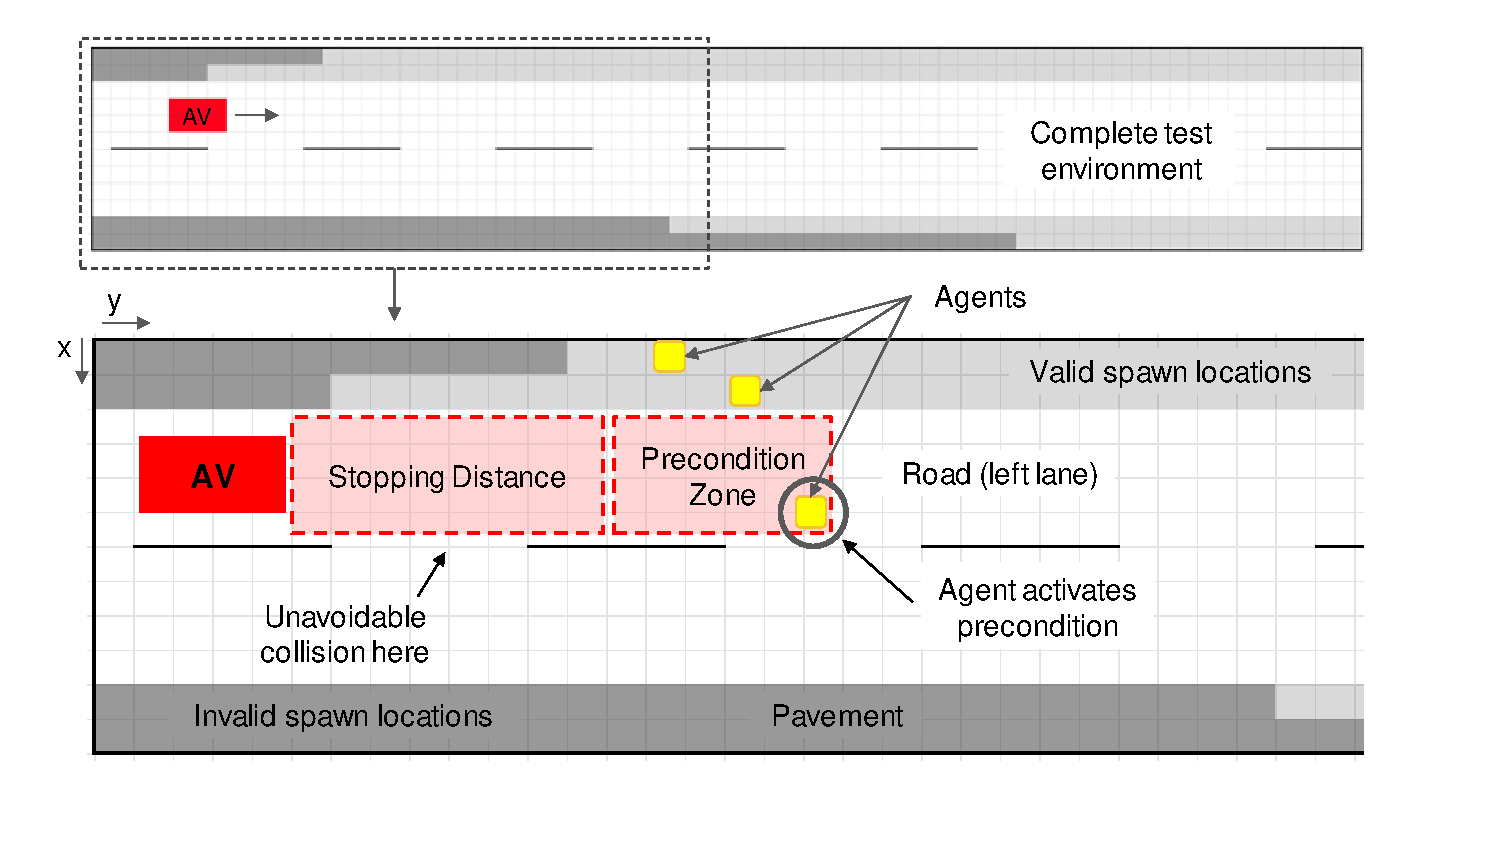
\includegraphics[width=0.54\textwidth]{RoadLayout.pdf}
	\caption{Test environment at full scale (upper part) and in detail (lower part), marking valid and invalid spawn locations for the pedestrians and indicating the position and direction of the AV (upper part).}
	\label{gridRoad}
\end{figure}


%------------------- Test Agents -----------------------------
\subsection{Test Agents}

The test agents in our case study are pedestrians. 
%
At the start of a test, pedestrians are randomly located onto the pavement area using valid spawn locations. The AV is a vehicle that drives at constant speed in a straight line, it does not brake or turn. For the purpose of comparing the performance of agent-based test generation techniques, the test agents have different behaviours from simple random (i.e.\ no direction through agency) to more directed, strategic planning-based agency, details of these are provided in this section.

We distinguish two main classes of behaviours, random and agency-directed, see also Table~\ref{t:ResultsTable}. For the random class, \textit{random} behaviour means that the test agent can perform any random action at each simulation tick, with the available actions being: do nothing (stand still), move forward, backward, left or right. In \textit{constrained random} mode, the pedestrian is initially walking along the pavement and has only one action available; to randomly choose when to cross the road. The constrained random behaviour is included so that a comparison between crossing the road at a targeted or at a random time can be made. 

The second class of behaviours is agency-directed, taking into account the agent's perceptions for strategic planning. Agents are initially walking along the pavement as in constrained random mode. The \textit{proximity} behaviour instructs the agent to cross the road when the AV is within a certain radius. The \textit{election} behaviour ranks agents within a proximity radius to the AV and elects the agent with the shortest distance to the AV. The major difference between the agent-directed behaviours is that the \textit{election} behaviour will only elect a single agent to cross the road whereas the \textit{proximity} behaviour will result any number of agents crossing the road as long as they are within range.
% Thus, the \textit{proximity} behaviour results in agents that will step into the road whenever a vehicle is nearby. Moreover, all nearby pedestrians are drawn to a passing vehicle.
%
While the \textit{proximity} behaviour may lead to the desired coverage it is less realistic than the \textit{election} behaviour. 
%
% The \textit{intersect} behaviour is more refined than the \textit{proximity} behaviour, but may still result in multiple agents attempting to intrude in the AV's \textit{precondition zone} simultaneously. 
%
% In contrast, the \textit{election} behaviour is designed to limit this to a single agent at a time.

% Agent numbers
The final factor to consider is the number of agents per test; too few and the likelihood of an agent activating the assertion will be low and entirely dependent on the initial starting position of the agent in the test environment due to differences in speed. The number of agents is physically limited by the number of available grid locations (1.5m spacing) on the pavement. % without overlap.
%
As the number of agents, $nA$, increases, it is expected that the probability of activating the assertion using a random behaviour increases significantly as more agents appear in the road, with a corresponding increase in computational expense. 
%
In comparison, when using more intelligent, agency-directed behaviour, we expect that with increasing $nA$, agents that can activate the assertion precondition are being generated more readily, thus resulting in shorter, less complex and hence more efficient tests. The range of $nA$ explored in this case study is from 1 to 20.

%------------------- Scoring -----------------------------
\subsection{Scoring}

In an attempt to encourage more realistic agent behaviour, a basic scoring system is used to direct agent behaviour by penalising or rewarding certain actions. In particular, a living cost of one is charged for each elapsed time step to promote shorter tests, and a penalty of five is issued for each time step that  an agent spends in the road. A reward of 100 is given if the agent enters the AV's \textit{precondition zone} More sophisticated scoring systems will be explored in our future work. 

% KIE: unclear :(
% The scoring should reflect the benefits of the method against the desire to generate good tests~\cite{fewster1999software}.



%------------------- Simulation and Logging -----------------------------
\subsection{Simulation and Logging}

Each agent behaviour was implemented in Jason~\cite{bordini2005jason} and executed within the testbench environment as described in Section~\ref{s:testbench}.
%
During simulation, the agents' actions, scores and time to test completion were recorded in a log.
% and then some statistics are compiled for each behaviour type. 

Each agent behaviour was repeated 1000 times and the number of successful tests was counted. A successful test is one that has a pedestrian intrude into the \textit{precondition zone} of the AV, thereby creating the opportunity for a subsequent intersection with the AV, i.e.\ a collision, thus triggering the AV's collision avoidance decision making logic.

%
A list of random start locations was created for the pedestrians for all settings of agent numbers, $nA$. This list was used to spawn the pedestrians for each of the agent behaviours to ensure the initial conditions between experiments were identical. 

%------------ Results Discussion ---------------
\section{Results}\label{s:results}
The results are evaluated based on five criteria; Accuracy is the ratio of successful tests the agents generated to the number of all tests, Score is a measure of how natural the agents behaved, Combined Score combines accuracy with score, Agent CPU Time is a measure of computational efficiency, and Test Generation Time is how long the agents took to generate the test in both simulation ticks and wall clock time. Both Score and Test Generation Time have distributions associated with them and therefore confidence intervals are provided.


%--------------------------------------------------------
\subsection{Test Accuracy}
Test accuracy, defined as the number of tests that have activated the precondition for the assertion as a ratio of all tests, is shown for each agent behaviour in Fig.~\ref{f:accuracy}. The \textit{random} and \textit{constrained random} behaviours have significantly lower accuracy compared to the directed agent behaviours when $nA<10$. For high $nA$ the accuracies converge mostly due to a saturation of agents in the test environment.
%
Fig.~\ref{f:accuracy} also shows that for $nA=1$ a directed agent outperforms a random agent by more than 2:1. The \textit{election} behaviour generates a slightly higher accuracy than the \textit{proximity} agent behaviour, but only by 2.2\%. However, for $nA=2$ and above the \textit{proximity} agent behaviour shows a 10\% increase in accuracy over the \textit{election} behaviour; this is because agents with this behaviour have multiple attempts to trigger the precondition whereas the election behaviour permits only one. 


\begin{figure}[!t]
	\centering
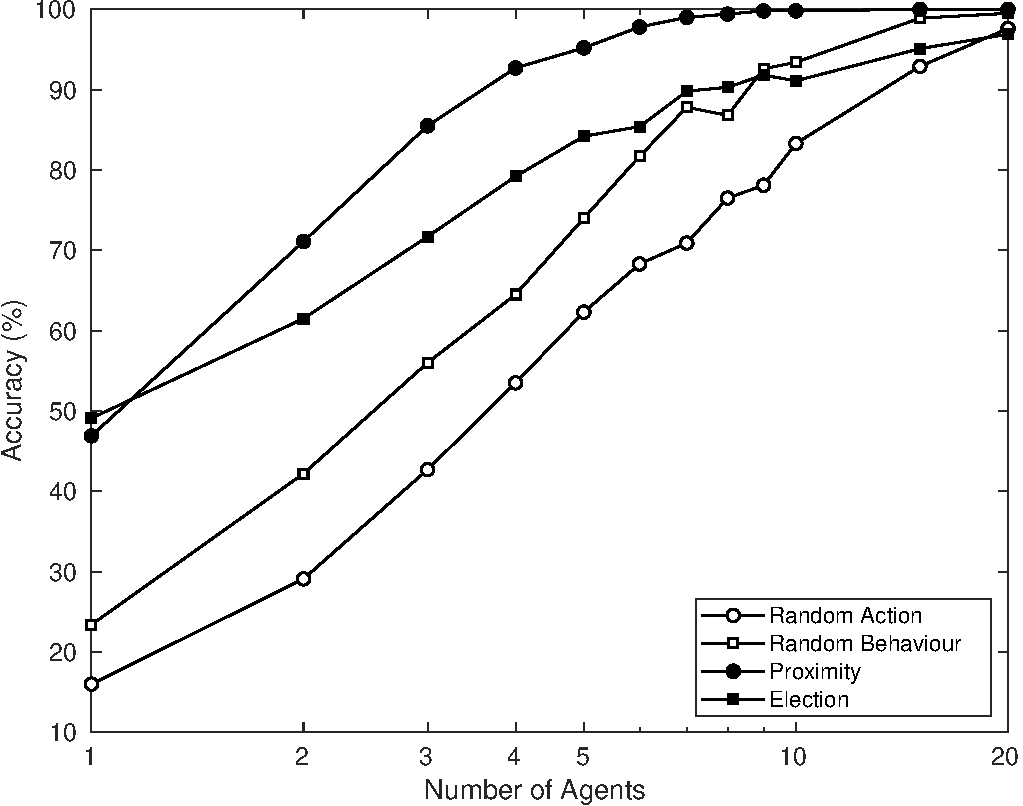
\includegraphics[width=0.48\textwidth]{Accuracy.pdf}
	\caption{Accuracy of agent behaviours to generate successful tests.}
	\label{f:accuracy}
\end{figure}


%--------------------------------------------------------
\subsection{Test Score} \label{s:testscore}

For tests that activate the precondition the average agent score is compiled including 95\% confidence intervals, see Fig.~\ref{f:agentscore}. The maximum theoretical score of any agent is 94, which includes 100 points for a successful test subtracting a living cost of one and a road penalty of five; this requires the agent to spawn adjacent to the \textit{precondition zone}. 
%
For a single agent, scores are similar for all agent behaviours, as only successful tests are included in the scoring. As the number of agents increases, the random behaviours diverge from the directed behaviours, and the variance observed for the random behaviour scores increases. This indicates that the directed agents display more natural behaviour than those using random.

% \todo[inline]{why no variance for nA=1 in random? this is counter intuitive, it suggests random agents that succeed score only the highest value score!} 

As $nA$ increases, the random agents are more often found in the road and hence their average score decreases. In contrast, the directed agents are only found crossing the road when they deem fit, and they remain on the pavement at all other times, keeping the score much higher and resulting in more realistic test cases.
%
% \todo[inline]{include the theoretical max score line} Note that the directed agent class are close to the theoretical maximum score, Fig.~\ref{AgentScore}(dashed line). 
%
% The high score for the $nA=1$ random class is surprising especially as the error bars are small indicating that, although the accuracy is low, tests generated are relatively efficient, i.e. the pedestrian does not spend a lot of time in the road.
%
No significant difference between the two directed behaviours can be observed in the score, even with a high number of agents. This indicates that  both result in similar level of realism in agent behaviour, at least within the limited scope of this example.


\begin{figure}[!t]
	\centering
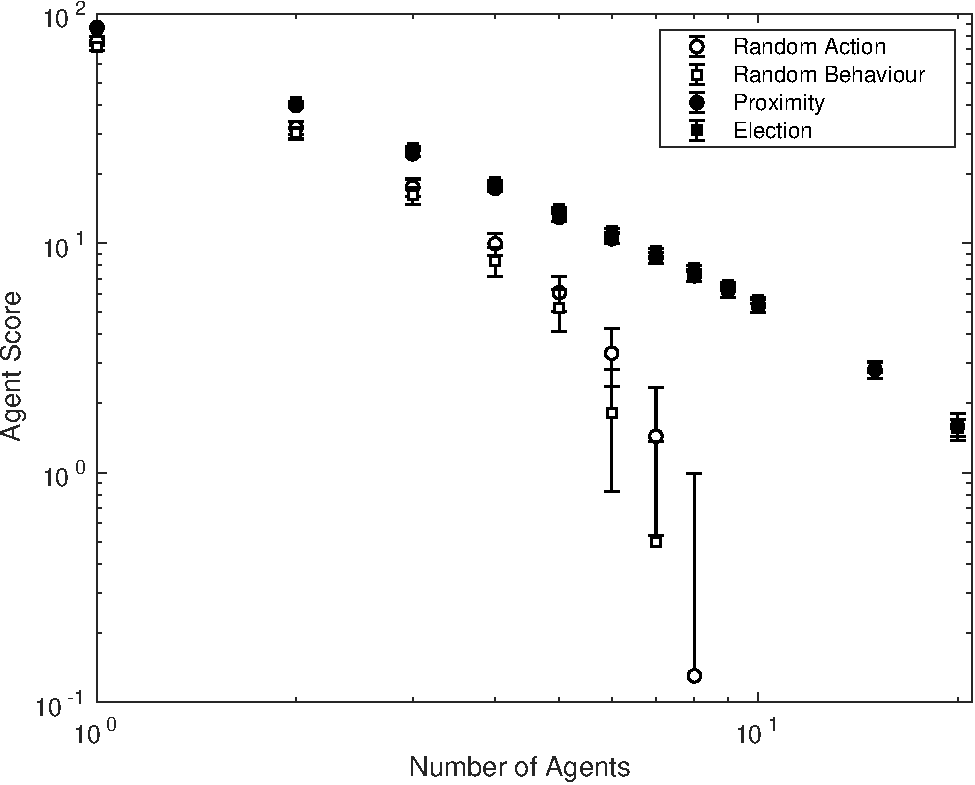
\includegraphics[width=0.48\textwidth]{AgentScore.pdf}
	\caption{The average agent score for successful tests with 95\% confidence intervals for each agent behaviour.}% Random class are hollow markers and directed class are filled. The maximum theoretical score is 94 points but this is only applicable to a single agent hence the declining average with increasing $nA$.}
	\label{f:agentscore}
\end{figure}


%--------------------------------------------------------
\subsection{Combined Score}
As the score in Section~\ref{s:testscore} only includes tests that meet the precondition, it is tempting to interpret these results as overly optimistic. To counteract this we use a \textit{combined score} that is calculated based on the score and accuracy using (score * accuracy / 1000). This combined measure promotes scores that are attached to high accuracies, describing agents that can generate successful tests with natural pedestrian behaviour. % Time could also ave been included as a denominator here but is already accounted for in the living cost penalty. %
%
The normalised results, Fig.~\ref{f:combined}, show that the directed agents are more than twice as effective within this new combined definition than agents with random behaviour for $nA=1$, although this lead drops rapidly with increasing agent numbers, reaching a steady performance gap of around 12\%.
%
The \textit{constrained random} agent behaviour outperforms the \textit{random} for $nA<4$ beyond which there is little difference. Therefore, if random behaviour is chosen, then the extra effort in implementing constrained random may not be worthwhile considering the low returns, except when using low agent numbers.
%
The \textit{election} agent behaviour has the highest combined score for $nA=1$, but as agent numbers increase, better results can be seen for the \textit{proximity} agent behaviour up to $nA=4$, beyond which there is no significant difference between the two directed agent behaviours.
%
% \todo[inline]{Describe relation to theoretical maximal?}

\begin{figure}[!t]
	\centering
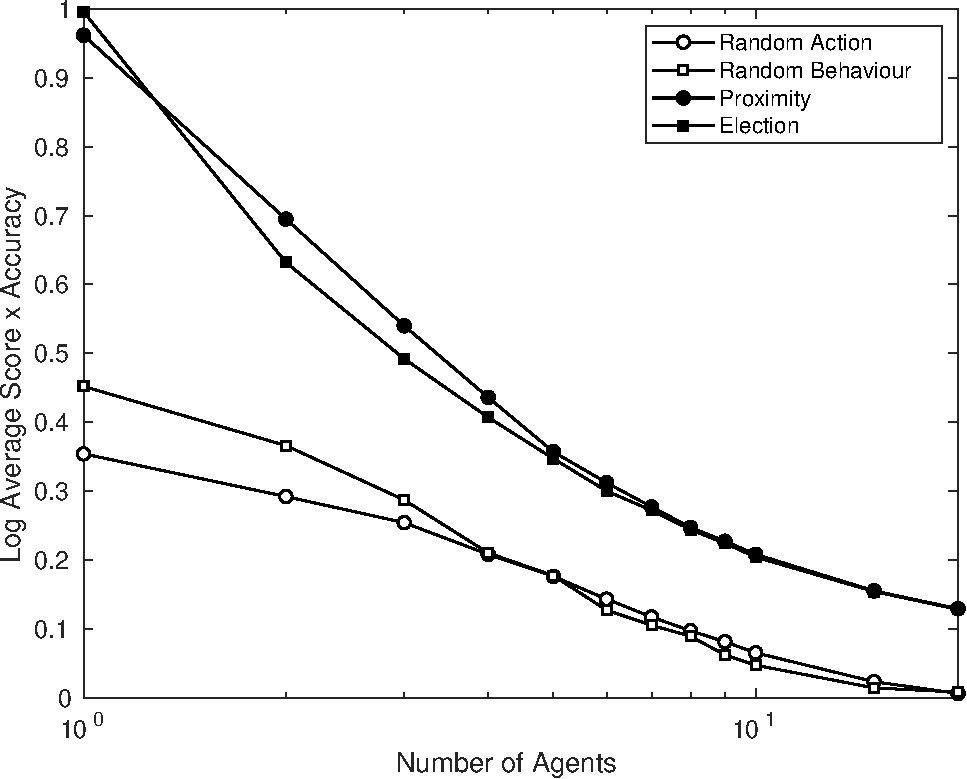
\includegraphics[width=0.48\textwidth]{Combined.pdf}
	\caption{The combined score including accuracy and the original score for each agent behaviour.}
	\label{f:combined}
\end{figure}

%\todo[inline]{y-axis is "normalised combined score" reduce height of all graphs by 30\%, change all x-axis to 1,2,3 not 10^0, add theoretical max score on this chart}


%--------------------------------------------------------
\subsection{Agent CPU Time}
% Metric of efficiency of the method, resource useage.
For each successful test, the CPU time used to execute the agent actions was averaged over the 1000 runs and assessed across different agent behaviours and numbers of agents, Fig.~\ref{f:cputime}. This allows comparing the resources required to execute agents of different behaviour types. The more complex agents have additional CPU overhead compared to agents with random behaviour. This difference remains relatively stable as agent numbers increase.

\begin{figure}[!t]
	\centering
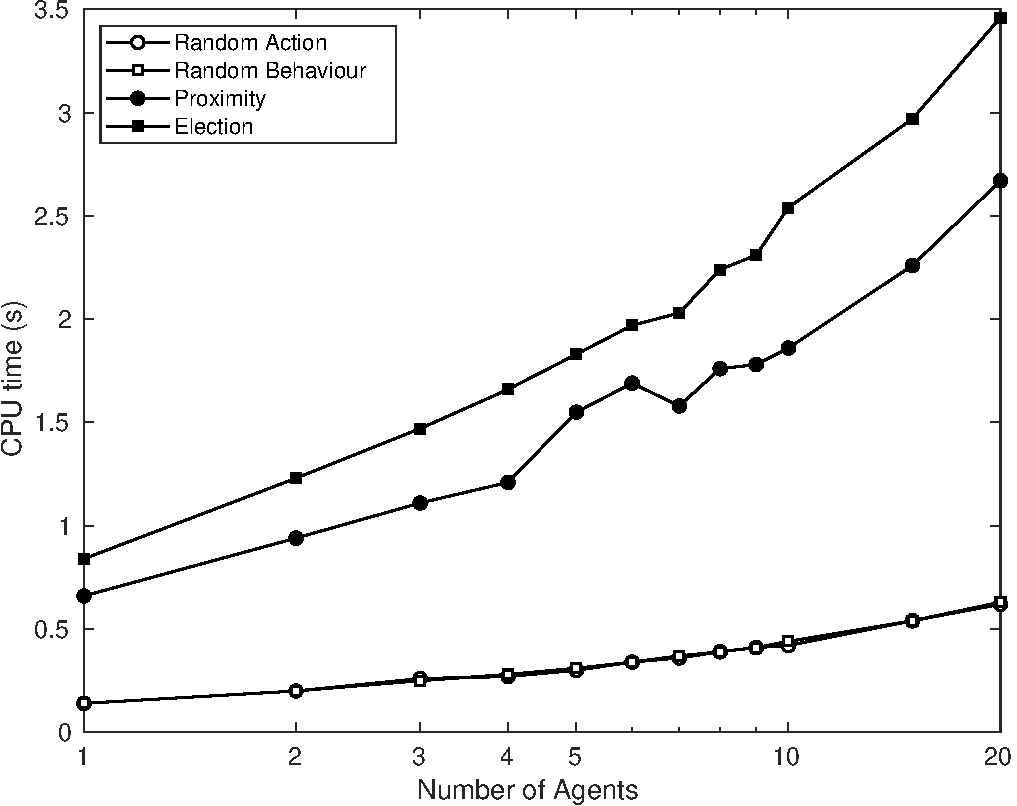
\includegraphics[width=0.48\textwidth]{TimeCPU.pdf}
	\caption{The CPU time, $t_{C}$, to execute agent actions averaged over 1000 runs.}
	\label{f:cputime}
\end{figure}

% \todo[inline]{change time y-axis to sim ticks not seconds, remove valid, add wall clock time to second y-axis, add error bars to time}


%---------------- Results Table -------------------------
\begin{table*}
\centering
\caption{Test agent summary table showing description and number of lines of code ($LOC$) for each agent and sample of results: Accuracy, Combined Score ($s_c$), CPU Time ($t_{c}$) and Test Generation Time ($t_{g}$) for $nA=3$.}
\label{t:ResultsTable}
\begin{tabular}{|l|p{7.1cm}|r||c|c|c|c|}
\hline
\textbf{Behaviour} & \textbf{Agent Description} & $LOC$ & Accuracy (\%) & $s_c$ (points)&  $t_{c}$ (s) & $t_{g}$ (ticks) \\
\hline
Random & Randomly perform action (forward, backward, left, right, stop) &  23& 42.7 & 0.254 & 0.09 & 9.11 \\
Constrained Random & Walk along pavement, randomly cross the road 		&  82& 56.0 & 0.287 & 0.08 & 8.83 \\
Proximity & Walk along pavement, cross road when AV in range 			&  86& 85.5 & 0.540 & 0.37 & 6.79 \\
Election & As in Proximity but elect a single agent to cross 			& 235& 71.7 & 1.470 & 0.49 & 6.59 \\
\hline 
\end{tabular}
\end{table*}


%--------------------------------------------------------
\subsection{Test Generation Time}
% Return on investment.
For each successful test generated, the number of simulation ticks consumed during test generation was averaged over 1000 runs and compared across different agent numbers for all four agent behavoiurs, Fig.~\ref{f:time}. 
%
The directed agents show improved performance over the agents with random behaviour for $nA=1$ by approximately a single simulation tick and this trend continues as agent numbers increase. By $nA=20$ the directed agents are 1.85 simulation ticks faster than the agents with random behaviour. Overall, the \textit{proximity} agents find tests in the smallest number of simulation steps.

\begin{figure}[!t]
	\centering
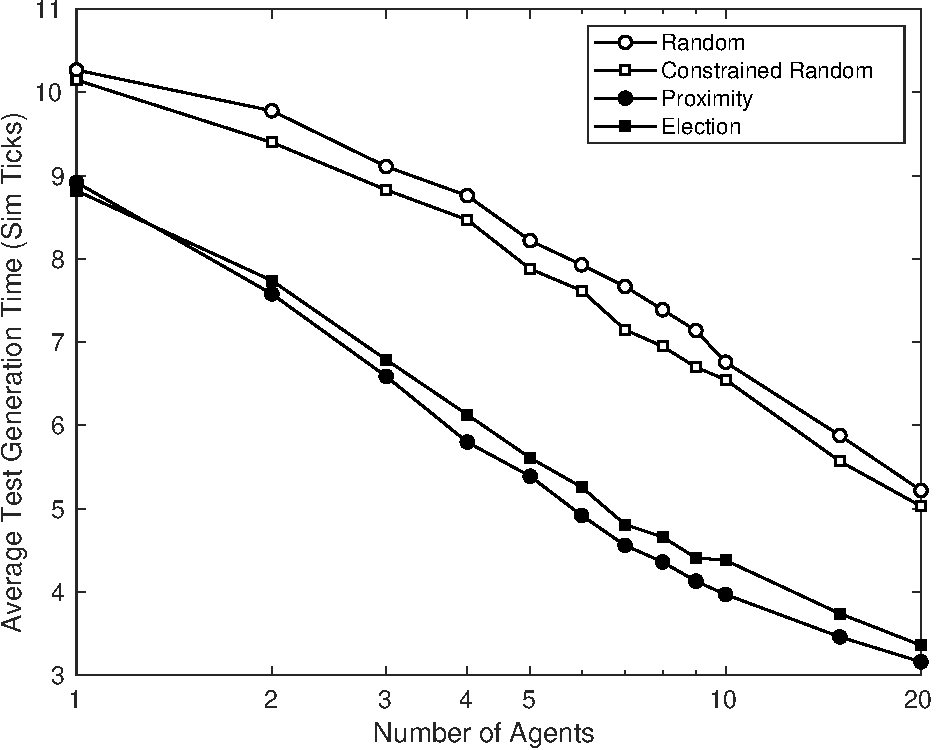
\includegraphics[width=0.48\textwidth]{TimeSimTicks.pdf}
	\caption{The average time taken for an agent to find a successful test, $t_{g}$.}
	\label{f:time}
\end{figure}

% \todo[inline]{change time y-axis to sim ticks not seconds, remove valid, add wall clock time to second y-axis, add error bars to time}



%--------------------------------------------------------
\section{Evaluation}\label{s:evaluation}
% \todo[inline]{discuss how the test show compliance against the `good test case' description in the intro: Accuracy is not precisely detecting defects in this case but the AV is put inot a situation where this is tested, Agent CPU is a resource metric = ecomonic, TTGT also economic but more a `return on investment' with efficiency. Agent score can be considered as the evolvable attribute as agents with a high score should do well in other environments (road layouts here) and still maintain realistic behaviour. The only attribute not covered is exemplary as in this case study only a single assertion is considered.}
% \todo[inline]{Agent density vs. accuracy - can be used to det how many agents required for map size}

% Shortcomings
% As with any model, refinements could be made to improve accuracy or reduce test generation time, such as choosing spawn locations and comparing direction of travel %between the AV and the agent or modifying pedestrian speed, but this example is kept simple to illustrate the concept. 

The results are assessed against the four criteria identified in Section~\ref{s:introduction}.

\textit{Effectiveness and Efficiency}: How effective is the method at generating tests that detect failures in the DUV, and how efficient is the method in minimising the number of tests required to achieve verification goals (i.e.\ assertion coverage)?
%
The accuracy metric, defined above, shows how often an agent generates a test that satisfies the precondition of the assertion, thereby triggering the execution of the AV's collision avoidance decision-making logic, creating the potential to reveal defects in the DUV and achieving assertion coverage in the process. 
%
Fig.~\ref{f:accuracy} shows that a small number of directed agents is around twice as effective as random ones and over three times as effective as a single agent.

%	\item \textit{Exemplary}: An exemplary test case will test the DUV against multiple assertions, an aspect of our future work, see Section~\ref{s:conclusion}. 
	% multiple aspects of the DUV thereby reducing the number of tests. In this case study, only a single assertion was used so this criteria cannot be assessed although it is a key development for future work discussed in Section~\ref{s:conclusion}.

\textit{Economy}: How costly is the test case to develop and run? %, analyse and debug? 
The resource cost (CPU time) to execute the agent actions, Fig.~\ref{f:cputime}, is 4-5 times higher for the directed agents than for agents with random behaviour, see also heading $t_{c}$ in Table~\ref{t:ResultsTable} for $nA=3$. %This may be a significant factor in the decision to use an intelligent agent unless abundant CPU resources are to hand. %
	%
	However, the test generation time ($t_g$), Fig.~\ref{f:time}, indicates that on average the directed agents find successful tests faster than random. Therefore, although more resource needs to be  allocated to the directed agents, overall they find test cases faster due to higher efficiency. %, leading to a higher return on investment.
%	
Wrt.\ development effort, the lines of code for each agent behaviour, see Table~\ref{t:ResultsTable}, show that for a moderate investment the \textit{random} behaviour can be improved significantly to obtain the performance of the \textit{proximity} behaviour. However, diminishing returns are evident beyond that. 
%
%To improve the combined score further with the \textit{election} agent took 10x the size of the \textit{random} code with lower overall accuracy but better combined score, suggesting this was not worth the investment.
%
% This also raises the question of how comlex the agents sould be? 
This simple scenario would suggest that the level of agent complexity should be considered carefully as a simpler level of agency could potentially be more beneficial than more complex options. 

\textit{Robustness} refers to the maintenance required to adapt tests to software changes, i.e.\ different \textit{scenes}. In the case study each test generated is of a different scene as the agent positions are randomly generated. The directed agents show higher robustness based on their accuracy when compared to random behaviours. 
%This is accounted for within the accuracy and could be easily shown to succeed with different road layouts and vehicle speeds, see Section~\ref{s:conclusion}.
% KIE: DO SO! (if it is easy)


% \todo[inline]{Do we need to add a new category to this list Eathly, Existent (def.=having reality), Embodied?-  level of natural or expected behaviour? Test cases generated may be both valid and interesting but not realistic - how do we control for this? do we need to? or does it not matter?}

% Further to this list of attributes, some generated tests may be \textit{valid} and \textit{interesting} but may not be \textit{realistic} i.e. a \textit{valid} test could technically happen but might never occur in reality. For example, a test that generated a vehicle driving in a river or parked on a building are invalid however a car driving the wrong way down a motorway/highway is valid but unrealistic. %
% \todo[inline]{Or is this just an example of an extreme edge case? Comments welome here as i'm not convinced of my own arguemnt! I suppose if you can you generate the same test in multiple ways then you should choose one that is more realistic.} %
% Therefore the category \textit{Existent} should be added:
% \begin{itemize}
% 	% \item \textit{Existent}: The level of reality of the test case beyond simply being valid. Agents in this case study are penalised for walking in the road, see Fig.~\ref{AgentScore}.
% 	% \item or...
% 	\item \textit{Existent}: Test cases should promote realistic scenarios or if competing valid cases exist then deference should be given to the more realistic one. Agents in this case study are penalised for walking in the road, see Fig.~\ref{AgentScore}.
% \end{itemize}


Overall, our results show that agency-directed testing outperforms random based, confirming that even a small amount of agency can be a distinct advantage over random techniques. 
%


%----------------- Conclusion ---------------------------
\section{Conclusion and Future Work}\label{s:conclusion}
The MAS programming paradigm offers rational agency, causality and strategic planning to software agents; these have been exploited in this research for test generation. 
%
On the example of a key assertion on collision avoidance we show that, by encoding a variety of different behaviours respondent to the agent's perceptions of the test environment, the agency-directed approach generates twice as many effective tests than a pseudo-random approach. Furthermore, agents can be encoded to behave more realistically without compromising their effectiveness. 
% I think this shouldbe changed  to state:
% Our results suggest that generating tests using testing agents allows engineers to reach edge cases and rare events more easily.
Our results suggest that generating tests using testing agents is a promising avenue of research and has been shown to significantly improves upon random whilst simultaneously providing more realistic driving scenarios.

Future work will extend this initial study to multiple assertions and a significantly larger variety of scenes including different road networks. 
As discussed in~\cite{Eder2007}, agents could have their goal selection modified based on coverage feedback, giving rise to  agent-based coverage-directed test generation. 
%
%would be an important step in this direction. This also 
%which fits in with the feedback reward of many such architectures, e.g. MDP~\cite{littman1994markov} and back-propagation for ANN~\cite{foerster2016learning}. %
%
Abstracting agent perceptions to a feature based representation could ensure the agent state space scales up to large physical maps and is adaptable to new features as more assertions are added.
Including personality in agents is also another avenue that could provide a tuning parameter~\cite{Zoumpoulaki2010} to generate edge cases. 
%Conventionally agressive (or egoist) behaviour may seem the most interesting as edge cases and therefore require oversampmling. But there could also be merit in exploring more risk-advers behaviours or simply in understanding what normative driving conditions are as a baseline for CAV cyber security. 
% There is also the possibility to have have combination of random and directed agents to ensure the initial 80\% of coverage is satisfied quickly then add more intelligent agents for hole coverage.


% : accuracy, cost and robustness. We want tests that are accurate (valid tests, collects coverage) and sufficiently low cost (CPU hours, engineering time). If tests are robust they are adaptable to real-time events, e.g. AV slows down around bend requiring agents to recalculate intersection.

%Robustness comes from the generated tests being adaptable to non-deterministic AV behaviour, i.e. linear extrapolation of the vehicle position is not possible. The origin of the graph below identifies the lowest cost, accuracy and robustness test cases which can be attributed to random generation. By using more advanced methods we hope to improve accuracy and robustness with minimal cost.




%----------------- Acknowledgment ---------------------------
\section*{Acknowledgement}
This research has in part been funded by the ROBOPILOT and CAPRI projects. Both
projects are part-funded by the Centre for Connected and Autonomous
Vehicles (CCAV), delivered in partnership with Innovate UK under grant numbers
103703 (CAPRI) and 103288 (ROBOPILOT), respectively.

% We gratefully acknowledge the support of NVIDIA Corporation with the donation of a Titan Xp GPU used for this research.

%----------------- Bibliography ---------------------------
\balance
\section*{References}
\printbibliography[heading=none]
\end{document}



% ensure readeris aware it is a fake AV not a real one
% map has non-traversible boundaries, no agents lost or created, define situation/scenario in terms of each test
% test can be regenerated exactly due to seed control
